% Options for packages loaded elsewhere
\PassOptionsToPackage{unicode}{hyperref}
\PassOptionsToPackage{hyphens}{url}
%
\documentclass[
  a4paper,
  twoside,
  12pt,
  chapterprefix=false,
  listof=flat]{scrartcl}
\usepackage{lmodern}
\usepackage{amssymb,amsmath}
\usepackage{ifxetex,ifluatex}
\ifnum 0\ifxetex 1\fi\ifluatex 1\fi=0 % if pdftex
  \usepackage[T1]{fontenc}
  \usepackage[utf8]{inputenc}
  \usepackage{textcomp} % provide euro and other symbols
\else % if luatex or xetex
  \usepackage{unicode-math}
  \defaultfontfeatures{Scale=MatchLowercase}
  \defaultfontfeatures[\rmfamily]{Ligatures=TeX,Scale=1}
\fi
% Use upquote if available, for straight quotes in verbatim environments
\IfFileExists{upquote.sty}{\usepackage{upquote}}{}
\IfFileExists{microtype.sty}{% use microtype if available
  \usepackage[]{microtype}
  \UseMicrotypeSet[protrusion]{basicmath} % disable protrusion for tt fonts
}{}
\makeatletter
\@ifundefined{KOMAClassName}{% if non-KOMA class
  \IfFileExists{parskip.sty}{%
    \usepackage{parskip}
  }{% else
    \setlength{\parindent}{0pt}
    \setlength{\parskip}{6pt plus 2pt minus 1pt}}
}{% if KOMA class
  \KOMAoptions{parskip=half}}
\makeatother
\usepackage{xcolor}
\IfFileExists{xurl.sty}{\usepackage{xurl}}{} % add URL line breaks if available
\IfFileExists{bookmark.sty}{\usepackage{bookmark}}{\usepackage{hyperref}}
\hypersetup{
  pdftitle={On the syntax of DP in Italian as non-native language},
  pdfauthor={Marco Petolicchio},
  hidelinks,
  pdfcreator={LaTeX via pandoc}}
\urlstyle{same} % disable monospaced font for URLs
\usepackage{longtable,booktabs}
% Correct order of tables after \paragraph or \subparagraph
\usepackage{etoolbox}
\makeatletter
\patchcmd\longtable{\par}{\if@noskipsec\mbox{}\fi\par}{}{}
\makeatother
% Allow footnotes in longtable head/foot
\IfFileExists{footnotehyper.sty}{\usepackage{footnotehyper}}{\usepackage{footnote}}
\makesavenoteenv{longtable}
\usepackage{graphicx,grffile}
\makeatletter
\def\maxwidth{\ifdim\Gin@nat@width>\linewidth\linewidth\else\Gin@nat@width\fi}
\def\maxheight{\ifdim\Gin@nat@height>\textheight\textheight\else\Gin@nat@height\fi}
\makeatother
% Scale images if necessary, so that they will not overflow the page
% margins by default, and it is still possible to overwrite the defaults
% using explicit options in \includegraphics[width, height, ...]{}
\setkeys{Gin}{width=\maxwidth,height=\maxheight,keepaspectratio}
% Set default figure placement to htbp
\makeatletter
\def\fps@figure{htbp}
\makeatother
\setlength{\emergencystretch}{3em} % prevent overfull lines
\providecommand{\tightlist}{%
  \setlength{\itemsep}{0pt}\setlength{\parskip}{0pt}}
\setcounter{secnumdepth}{5}
%\usepackage[a4paper,left=4.5cm, top=3.5cm, bottom=3.5cm, right=4.5cm, heightrounded, headsep=2em, footskip=11mm, vmarginratio=1:1]{geometry}
\usepackage[a4paper,margin=4cm,  heightrounded, headsep=2em, footskip=11mm, vmarginratio=1:1]{geometry}
\makeatletter
\DeclareOldFontCommand{\rm}{\normalfont\rmfamily}{\mathrm}
\DeclareOldFontCommand{\sf}{\normalfont\sffamily}{\mathsf}
\DeclareOldFontCommand{\tt}{\normalfont\ttfamily}{\mathtt}
\DeclareOldFontCommand{\bf}{\normalfont\bfseries}{\mathbf}
\DeclareOldFontCommand{\it}{\normalfont\itshape}{\mathit}
\DeclareOldFontCommand{\sl}{\normalfont\slshape}{\@nomath\sl}
\DeclareOldFontCommand{\sc}{\normalfont\scshape}{\@nomath\sc}
\makeatother




\usepackage{fontspec}

\usepackage{ifluatex}

\usepackage{microtype}



\setmainfont[Numbers=Lowercase]{IBMPlexSerif}
\setsansfont[Numbers=Lowercase]{IBMPlexSans}
\setmonofont[Numbers=Lowercase, Scale=.8]{IBMPlexMono}


\usepackage[english]{babel}





\usepackage[all]{nowidow}






\definecolor{upol-dGrey}{rgb}{0.36470588235,0.36862745098,0.37647058823}
\definecolor{upol-lGrey}{rgb}{0.8,0.8,0.8}
\definecolor{upol-brandBlue}{rgb}{0,0.43529411764,0.67843137254}


\usepackage{xcolor}
\usepackage{graphicx}
\definecolor{titlepagecolor}{cmyk}{1,.38,0,.15} %C100 M38 Y0 K15
\definecolor{namecolor}{cmyk}{0, 0, 0, .0980} 
\usepackage{textcase}


\usepackage{setspace}

\makeatletter\let\Title\@title\makeatother
%\makeatletter\let\Author\@author\makeatother



\usepackage{sectsty}
\allsectionsfont{\color{upol-dGrey}\sffamily}
\chapterfont{\color{upol-dGrey}\raggedleft\thispagestyle{empty}}





\usepackage{floatrow}
\floatplacement{figure}{!ht}
\floatplacement{table}{!ht}
\floatsetup[table]{font=sf}
\floatsetup[figure]{font=sf}
\floatsetup[tikzpicture]{font=sf}

\usepackage[font={color=upol-dGrey}, labelfont={color=upol-dGrey}]{caption}



\makeatletter
\def\verbatim@font{\linespread{1}\footnotesize\ttfamily}
\makeatother



\makeatletter
\renewenvironment{figure}[1][\fps@figure]{
  \edef\@tempa{\noexpand\@float{figure}[#1]} 
  \@tempa
  \sffamily
}{
  \end@float
}
\renewenvironment{table}[1][\fps@table]{
  \edef\@tempa{\noexpand\@float{table}[#1]} 
  \@tempa
  \sffamily
  \footnotesize
}{
  \end@float
}
\makeatother

\usepackage{tabularx,tabu}
\usepackage{amsfonts}
\usepackage{booktabs}
\usepackage{siunitx}
\usepackage{fancyhdr}

\usepackage{lipsum, kantlipsum} % just for testing

\pagestyle{fancy}
\fancyhf{}
\fancyhead[LE,RO]{\thepage}
%\fancyhead[RE]{\footnotesize\nouppercase{\leftmark}}
\fancyhead[RE]{\footnotesize\nouppercase{M. Petolicchio, \textit{DPs Syntax in acquisition}}}
\fancyhead[LO]{\footnotesize\nouppercase{\rightmark}}
\setlength{\headheight}{14.5pt} % as requested by fan
\renewcommand{\headrulewidth}{0pt}

%\renewcommand{\chaptermark}[1]{\markboth{\thechapter \ . \  #1}{}}
\renewcommand{\sectionmark}[1]{\markright{\thesection \ \ #1}{}}





%\setcounter{secnumdepth}{5}
%\setsecnumdepth{subsubsection}
%\maxtocdepth{subsubsection}


\setlength{\skip\footins}{3em}
\renewcommand\footnoterule{{\hrule height 0pt}} % a long blue line



\usepackage{colortbl}
\arrayrulecolor{gray}







\usepackage{booktabs}

\usepackage{pdfpages}






%Options: Sonny, Lenny, Glenn, Conny, Rejne, Bjarne, Bjornstrup
\usepackage[Bjornstrup]{fncychap}
%\renewcommand{\CNoV}{\raggedleft\sffamily\selectfont\HUGE}
  \ChNumVar{\Huge\sffamily\selectfont}
\renewcommand{\DOCH}{%
   \settowidth{\py}{\CNoV\thechapter}
  \addtolength{\py}{1em}      % Amount of space by which the
%                                % number is shifted right
   \fboxsep=0pt%
   \colorbox[gray]{.85}{\rule{0pt}{50pt}\parbox[b]{\textwidth}{\hfill}}%
   \kern-\py\raise20pt%
   \hbox{\color{gray}\CNoV\thechapter}\\%
}

\makeatletter
\renewcommand*{\@makechapterhead}[1]{%
  \vspace*{0\p@}%
  {\parindent \z@ \raggedright \normalfont
    \ifnum \c@secnumdepth >\m@ne
      \if@mainmatter%%%%% Fix for frontmatter, mainmatter, and backmatter 040920
        \DOCH
      \fi
    \fi
    \interlinepenalty\@M
    \if@mainmatter%%%%% Fix for frontmatter, mainmatter, and backmatter 060424
      \DOTI{#1}%
    \else%
      \DOTIS{#1}%
    \fi
  }}
% For the case \chapter*:
\renewcommand*{\@makeschapterhead}[1]{%
  \vspace*{10\p@}%
  {\parindent \z@ \raggedright
    \normalfont
    \interlinepenalty\@M
    \DOTIS{#1}
    \vskip 0\p@
  }}
\makeatother





\usepackage{tikz,tikz-qtree}


\tikzstyle{every picture}+=[font=\sffamily]

\usepackage{listings}
\lstset{ %Formatting for code in appendix
	backgroundcolor = \color{gray},
	language=Python,
	basicstyle=\singlespacing\footnotesize\ttfamily\color{white},
	numbers=left,
	stepnumber=1,
	showstringspaces=true,
	tabsize=2,
	breaklines=true,
	breakatwhitespace=false,
	xleftmargin=3em,framexleftmargin=3em, numberstyle=\ttfamily,
}

\usepackage{datetime}

%\let\oldmaketitle\maketitle
%\AtBeginDocument{\let\maketitle\relax}




\usepackage{catchfilebetweentags}

\usepackage[autostyle]{csquotes}  
\usepackage{enumerate}


\makeatletter
\newcommand\HUGE{\@setfontsize\Huge{36}{48}} 
\makeatother

\usepackage{tikz}
\usepackage{pgfplots}


\usepackage{gb4e,cgloss}
\noautomath
\let\eachwordone=\itshape


\usepackage{amsthm}

\theoremstyle{plain} % default
\newtheorem{theorem}{Theorem}[section]
\newtheorem{lemma}[theorem]{Lemma}
\newtheorem{proposition}[theorem]{Proposition}
\newtheorem*{corollary}{Corollary}

\theoremstyle{definition}
\newtheorem{definition}{Definition}[section]
\newtheorem{conjecture}{Conjecture}[section]
\newtheorem{example}{Example}[section]
\newtheorem{postulate}{Postulate}[section]
\newtheorem{problem}{Problem}[section]

\theoremstyle{remark}
\newtheorem*{remark}{Remark}
\newtheorem*{note}{Note}
\newtheorem{case}{Case}


\usepackage{float}
\usepackage[]{natbib}
\bibliographystyle{apa}

\title{On the syntax of DP in Italian as non-native language}
\usepackage{etoolbox}
\makeatletter
\providecommand{\subtitle}[1]{% add subtitle to \maketitle
  \apptocmd{\@title}{\par {\large #1 \par}}{}{}
}
\makeatother
\subtitle{A case study on Czech and Slovak learners}
\author{Marco Petolicchio}
\date{}

\begin{document}
\maketitle
\begin{abstract}
This study aims to investigate over the internal syntax of Noun phrases in non-native Italian by Czech and Slovak learners. The typological difference in those languages are used to reconnect with the generative models on language acquisition, while the linguistic data is threated quantitatively to show the gap between L2 production and the standard behaviour in mono-lingual corpora.

\par

\textbf{Keywords:} Corpus linguistics, Determiner phrase, Italian L2, Second language acquisition, Syntax
\end{abstract}

{
\setcounter{tocdepth}{2}
\tableofcontents
}
\clearpage

\hypertarget{introduction}{%
\section{Introduction}\label{introduction}}

Czech (\texttt{ces}) and Slovak (\texttt{slk}) are languages of the Slavic branch in the Indo-european family. Alongside a certain morphological complexity in noun declension systems, these languages --except for Bulgarian (\ref{exm:dpBul}) and Macedonian \citep{wals-37}-- don't show an overt realization of the Determiner position inside the noun phrase (\ref{exm:dpNo}) \citep{harkins1953}.
Conversly, Italian (\texttt{ita}) and the other romance languages explicit that position as a default behaviour, usually with a free morpheme preceding the noun (\ref{exm:dpPre}) or by cliticization of the definite article (\ref{exm:dpRon}):

\begin{enumerate}
\def\labelenumi{(\arabic{enumi})}
\tightlist
\item
  Articleless \label{exm:dpNo}

  \begin{enumerate}
  \def\labelenumii{\alph{enumii}.}
  \tightlist
  \item
    \texttt{ces} \citep[ 14]{veselovska2014}\\
    \gll    Chlapec/Marie/Ona/každý miluje ryby/ \{své rodiče\}.\\
    Boy/Marie/She/Everyone Love.3sg Fish/ \{POSS parent\}\\
    \glt    \enquote{SUBJ loves {[}the{]} fish/ his parents}
  \item
    \texttt{slk} \citep[ 113]{krizomkrazomA1}\\
    \gll    Večer čítam knihy, píšem referáty\ldots{}\\
    Evening Read.1SG Book.PL Write.1SG Paper.PL\\
    \glt    \enquote{In the evening I read {[}the{]} books, I write (school) papers \ldots{}}
  \end{enumerate}
\item
  Proclitic \label{exm:dpPre}

  \begin{enumerate}
  \def\labelenumii{\alph{enumii}.}
  \tightlist
  \item
    \texttt{ita} \citep[ 60]{bianco2017}\\
    \gll    Il terremoto ha distrutto la città.\\
    ART.DEF Earthquake AUX.3sg Destroy.PTCP.PST ART.DEF City\\
    \glt    \enquote{The earthquake destroyed the city}
  \item
    \texttt{fro} \citep[ 3261]{dedole2008}\\
    \gll    La dame estoit devant la sale.\\
    ART.DEF Girl Be.3sg ADV ART.DEF Room\\
    \glt    \enquote{The \emph{dame} was in front to the room}
  \end{enumerate}
\item
  Enclitic

  \begin{enumerate}
  \def\labelenumii{\alph{enumii}.}
  \tightlist
  \item
    \texttt{ron} \citep[ 45]{cojocaru2003} \label{exm:dpRon}\\
    \gll    Prieten=ul meu este aici.\\
    Friend=ART.DEF POSS Be.PRES.3sg Here\\
    \glt    \enquote{My friend is here}
  \item
    \texttt{bul} \citep[ 37]{leafgren2011} \label{exm:dpBul}\\
    \gll    Къде е книга=та ми?\\
    Where Be.3SG Book=ART.DEF POSS.1SG\\
    \glt    \enquote{Where is my book?}
  \end{enumerate}
\end{enumerate}

The general idea of this paper is to address the question of how linguistic structures which are not overtly marked in L1 can be accessed during the acquisition of a target language which show them. While doing this can be either both purely speculative and meanwhile grounded on actual data, I will show how the usage of a targeted linguistic corpora which can be useful to concentrate the main hypotheses into narrower facts. The language under observation are manifold: on one side Czech (\texttt{ces}) and Slovak (\texttt{slk}) as native languages--with no position for the articles--with Italian (\texttt{ita}) on the other side as the target language.

The section \ref{sec:theoryBg} provides a theoretical discussion on the top of different theories inside the generative framework \citep{chomsky1995} on the status of DP and NP. The section \ref{sec:caseStudy} is twofold: firstly I present the methods used into the current study in terms of \emph{reproducibility} of research and an analysis of the expected results; while the second subsection is built upon a case study made test hypotheses about the categorial differences of DPs during the acquisition of \texttt{ita} by \texttt{ces} and \texttt{slk} native speakers involved in the test.
A summary conclusion (Section \ref{sec:concl}) closes the paper.

\hypertarget{sec:theoryBg}{%
\section{Theoretical background}\label{sec:theoryBg}}

\hypertarget{the-generative-view-on-language}{%
\subsection{The generative view on language}\label{the-generative-view-on-language}}

From a generative-oriented point of view, the human language is a computational procedure which relies on a hierarchical organization of structures, and language variations are connected to a parametrizing of choice among those structures \citep{adger2013, chomsky1995, chomsky1998, chomsky2013, chomsky2015, rizzi2013}:

\begin{quote}
We are concerned, then, with states of the language faculty, which we understand to be some array of cognitive traits and capacities, a particular component of the human mind/brain. The language faculty has an initial state, genetically determined; in the normal course of development it passes through a series of states in early childhood, reaching a relatively stable steady state that undergoes little subsequent change, apart from the lexicon. To a good first approximation, the initial state appears to be uniform for the species. \citep{chomsky1995}
\end{quote}

From this perspective, the possibility of comparation is offered either by different languages or among different states of language acquisition: structures can be compared and analysed into a coherent grid in order to perform further analyses and reveal similarities and differences in the parametrizing of syntax.

\hypertarget{the-role-and-the-study-of-interlanguage}{%
\subsection{The role and the study of interlanguage}\label{the-role-and-the-study-of-interlanguage}}

For many scholars the role of the native language (L1) carries possible conditioning for the way which the target language (L2) is acquired during the path to learning: an emblematic case is the \emph{transfer} of the knowledge about the structures of the L1 to the target, revealing the intermediate steps of the acquisitional path, which is the hypothesis of \emph{interlanguage} addressed by Selinker \citep{selinker1972}.
One of the main areas of research in Generative Studies on Second Language Acquisition (\texttt{GenSLA}) regards investigating how linguistic structures can be accessed in L2 and how the transitional stages of acquisition work into the learning \emph{continuum} \citep{rothmanslabakova2017}.

During the last 20 years, a considerable part of linguistic activity has been involved in developing some sort of models to describe how the faculty of language works, through its biological \citep{hcf2002}, computational \citep{fodor2001} and cognitive components in a highly interdisciplinary environment.
SLA is a fertile field, which relies on the comparative and contrastive analyses of linguistic phenomena, either both from an applied view \citep{ellis1994} or by theoretically grounded perspective focused on GenSLA \citep{guasti2002, hawkins2001, rothmanslabakova2017, sorace2011}.

\hypertarget{the-position-of-dp-and-np}{%
\subsection{The position of DP and NP}\label{the-position-of-dp-and-np}}

There are striking differences between languages that display an overt D position and those that do not in respect to the syntactic behaviour of NP, as such as Left Branch Extraction allowing, scrambling or adjective extraction. Those properties are summarized in the table below \citep[in][ from \citet{boskovic2009}]{salzmann2018}:

\begin{longtable}[]{@{}lll@{}}
\caption{Typology of Overt D vs.~Covert D languages}\tabularnewline
\toprule
& Overt D & Covert D\tabularnewline
\midrule
\endfirsthead
\toprule
& Overt D & Covert D\tabularnewline
\midrule
\endhead
allow adj extraction from NP & no & yes\tabularnewline
allow LBE & no & yes\tabularnewline
allow Neg-raising & yes & no\tabularnewline
allow scrambling & no & yes\tabularnewline
allow the majority superlative reading & yes & no\tabularnewline
allow trans. nominals with 2 non-lex. genitives & yes & no\tabularnewline
can be polysynthetic & no & yes\tabularnewline
island sensitivity in head-internal relatives & no & yes\tabularnewline
superiority effect in wh-mvt & yes & no\tabularnewline
\bottomrule
\end{longtable}

Since Abney's seminal work \citep{abney1987} there two hypotheses have been established to represent this structure: (i) NP-over-DP, for which the DP is at the edge of NP as specifier; (ii) DP-over-NP, where the DP dominates the NP:

\begin{figure}

{\centering 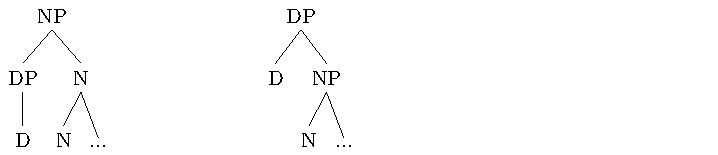
\includegraphics[width=1\linewidth]{_main_files/figure-latex/tree1-1} 

}

\caption{Phrase structure in NP-over-DP vs. DP-over-NP Hypotheses}\label{fig:tree1}
\end{figure}

Following this approach \citep{abney1987}, in generative studies it is assumed that nouns project a higher functional category--Determiners--with their phrase DP, wherein a restricted class of items can be (articles, quantifiers etc.).
The \emph{DP Hypothesis} aims to reconnect the internal geometry of the Determiner Phrase to the generalized phrase structure of complex elements \citep{bernstein2008, zamparelli1995} for which, independent of the actual presence of DP elements on a morphological level, the functional category of DP is still in the derivation.

\hypertarget{sec:caseStudy}{%
\section{The analysis of data}\label{sec:caseStudy}}

\hypertarget{the-datasets}{%
\subsection{The datasets}\label{the-datasets}}

For the analysis of \texttt{ita} as a non-native language for \texttt{ces} and \texttt{slk} learners, the 3 corpora below have been subsetted and collected into a dataframe (henceforth \enquote{\emph{collection}}):

\begin{itemize}
\item
  \textbf{\href{http://www.valico.org/valico_b_CORPUS.html}{GranVALICO}} and \textbf{\href{http://www.valico.org/valico_CORPUS.html}{VALICO}} \citep{valico}\\
  Learner corpora provided by Turin University. They represent the most valuable sources of Italian L2 corpora. They are composed by written texts composed by the students which have the assignment to describe vignettes provided by the teachers. The corpora are accessible online with an advanced search that permits filtering the data along different parameters (e.g.~learners' L1 and education, assignments etc.).
\item
  \textbf{\href{http://merlin-platform.eu}{MERLIN}} \citep{merlin}\\
  The MERLIN Corpus is a wide-ranging multilingual documented resource which collects 2.286 texts written by learners of Czech, Italian and German.
  Started in 2012, the main objective is to show the different levels of language acquisition using written texts, relying on the CEFR level schema on L2 acquisition.
  The Italian-L2 subcorpus contains 813 texts.
\item
  \textbf{\href{http://czech-it.github.io}{Czech-IT}} \citep{czech-it}\\
  The Czech-IT corpus contains chat messages, emails, conversations, surveys and assignments by more than 70 Czech and Slovak learners of Italian language.
  Started in 2017, it is fully accessible online.
\end{itemize}

Additionally, two monolingual L1 corpora have been used for \texttt{ita} and \texttt{ces}:

\begin{itemize}
\item
  \textbf{\href{http://books.google.com/ngrams}{Google nGram Viewer Italian}} \citep{ngram2011}\\
  With more than 40 billions words with an estimated accuracy rate of 95.6\% for POS-tagging and 80.0\% for dependency parsing \citep{ngram2012}, the Italian corpus represents a wide collection of data to study monolingual \texttt{ita} in written form. Developed at Google, the nGram Viewer presents an interface to deal with those corpora in a standalone way.
\item
  \textbf{\href{http://ucnk.korpus.cz/syn2010.php}{Syn2010}} \citep{syn2010}\\
  Part of the a documentation project of the Czech National Corpus (CNK, \emph{Český Národní Korpus}), SYN2010 is a representive corpus of contemporary Czech writing containing more than 100 million words, which includes texts of fiction (40\%), journal articles (27\%), and professional literature (33\%).
\end{itemize}

\hypertarget{methods}{%
\subsection{Methods}\label{methods}}

The data from the three corpora have been subsett for analysis, including only the data which present \texttt{ita} as the target language by \texttt{ces} and \texttt{slk} learners and merged into a collection which consists of 411 texts and 35391 tokens.
The texts in the collection are computationally processed in sequential steps in order to retrieve a comparable basis for data analyses. In the first step, only the relevant pieces were extracted from their original dataset and then they were processed towards the use of the library UDPIPE \citep{udpipe2017} in R. The corpora were cleaned by the deletion of non-informative structures (e.g.~punctuation marks), and merged (Table \ref{tab:tableCollection}):

\begin{table}[t]

\caption{\label{tab:tableCollection}\label{tab:tableCollection}Structure of data in the collection}
\centering
\begin{tabu} to \linewidth {>{\raggedright}X>{\raggedright}X>{\raggedright}X>{\raggedright}X>{\raggedright}X}
\toprule
\multicolumn{1}{c}{ } & \multicolumn{2}{c}{Texts} & \multicolumn{2}{c}{Tokens} \\
\cmidrule(l{3pt}r{3pt}){2-3} \cmidrule(l{3pt}r{3pt}){4-5}
  & ces & slk & ces & slk\\
\midrule
Czech-IT & 212 & 74 & 11129 & 4440\\
Merlin & 1 & 0 & 256 & 0\\
Valico & 107 & 17 & 16250 & 3316\\
\bottomrule
\end{tabu}
\end{table}

Additionally, mono-lingual data were been analysed for comparison. For the Czech language, the analysis relies on the work of Veselovská \citep{veselovska2014} based on SYN2010 \citep{syn2010}. The statistics on the Italian corpus were been provided by the submission of syntactic queries against the Google NGram API \citep{ngram2011} on Google Books ITA (1500-).

\hypertarget{results}{%
\subsection{Results}\label{results}}

The data in the collection was computationally processed in order to retrieve quantitative information about the overall distribution of the syntactic phrase, specifically elicited in the environments that present a Noun element. These clusters were been analysed by their condition in the environment, giving the possibility to compare the distribution of single tags in the antecedent position of a noun or in the subsequent position.
A general POS tagging pipeline was established with the usage of the free library UDPIPE for R. While those tools reach far beyond 90\% accuracy in POS-tagging for mono-lingual corpora, it was also determined that learner-based corpora posit a challenge for automated tasks.

The chart below (Figure \ref{img:2gramCollection}) presents the occurrence of bigrams clustering with N, extracted from the collection of corpora.

\begin{figure}
\centering
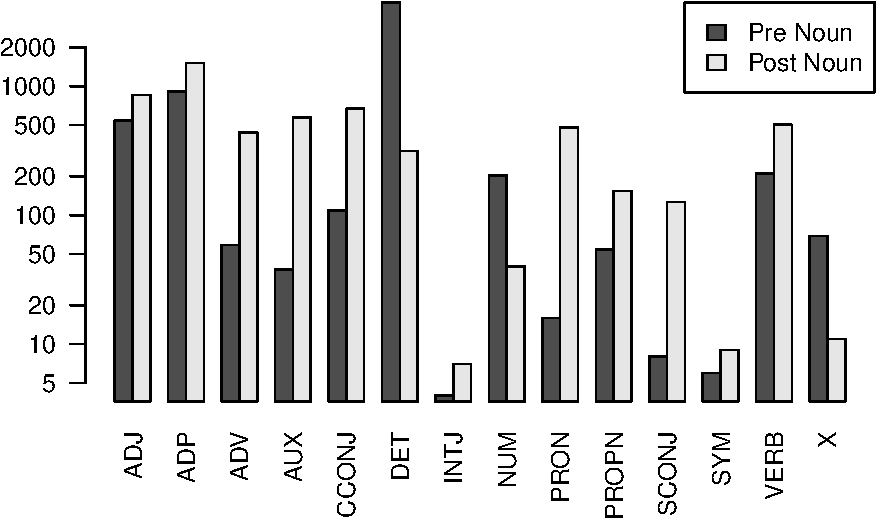
\includegraphics{_main_files/figure-latex/graphNoun-1.pdf}
\caption{\label{fig:graphNoun}\label{img:2gramCollection}Distribution of 2-grams with N in Collection}
\end{figure}

Additionally, SYN2010 and Google NGram data were compared to the collection.\\
While the analysis of the SYN2010 corpus relied on the study by Veselovská \citep{veselovska2014} except for the statistics of ADP+N/N+ADP clusters, results yielded by the diachronic analysis on Google nGram were processed by their central tendency, calculated by the arithmetic mean (AM).
With a data set containing the values \texttt{a\_1,a\_2,\ldots{},a\_n} thus the arithmetic mean is defined by the formula:

\begin{equation}
    AM=\frac{1}{n}\sum_{i=1}^n a_i = \frac{a_1 + a_2 + \ldots + a_n}{n} 
\end{equation}

The amounts of the clusters in the dataset were weighted by their absolute distribution and refactored to a value equal to 1. The plot below (Figure \ref{img:2gramTotal}) shows the close comparison of these clusters in the dataset\footnote{The category of DET in SYN2010 corresponds to DEM, Q, PRON (not POSS) \citep[20]{veselovska2014}.}.

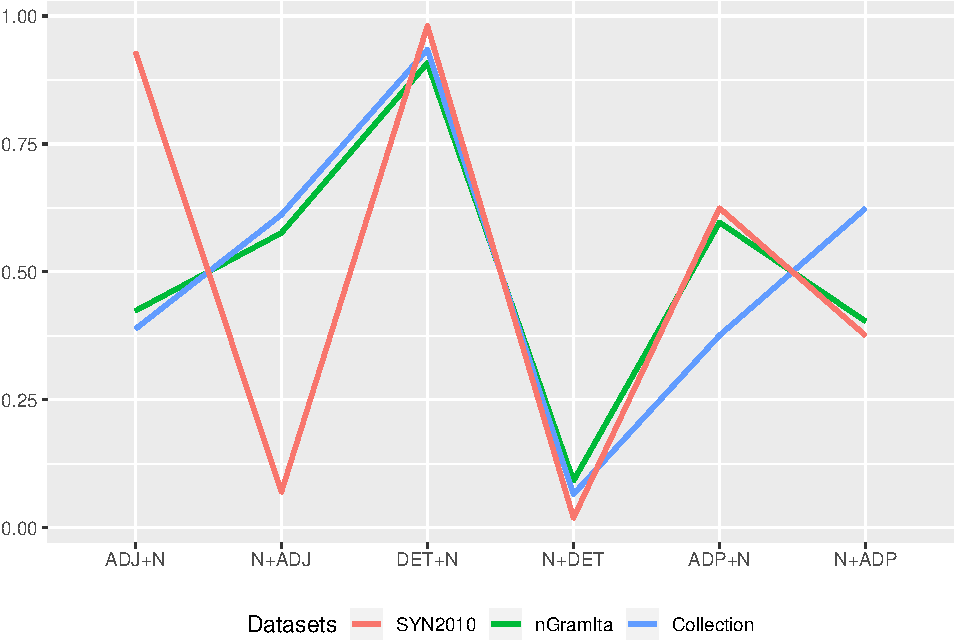
\includegraphics{_main_files/figure-latex/corporaNoun-1.pdf}
The presented data does not deal directly with the problem of evaluating the automated tasks involved in the process, and had to be cleared out indicating that there can be some weaknesses in the usage of mono-lingual trained processors in learner corpora. Moreover, while these can be implemented towards an application in multilingual contexts, it appears that an overall application of this process cannot be done flawlessly since the complexity of the language acquisition path. Also, the differing sizes of the corpora involved in the analysis, which display different magnitude of breadth (nGram is over 40 billion of tokens, the collection 39 thousand), and plays a role in the analysis of the data itself.

In this sense it appears that a certain tendency can be seen in the examples discussed above. While it shows a certain uniformity in the absolute value of DET-N clusters in the dataset, a major shift arises in the position of the adjectives, which can be traced by the typological differences among the languages under analysis:

\begin{enumerate}
\def\labelenumi{(\arabic{enumi})}
\setcounter{enumi}{3}
\item
  \begin{enumerate}
  \def\labelenumii{\alph{enumii}.}
  \tightlist
  \item
    \texttt{ces} \label{exm:adjCes}\\
    \gll    To červené auto.\\
    DEM.NT ADJ.NT NOUN.NT\\
    \glt    \enquote{That red car}
  \item
    \texttt{ita} \label{exm:adjIta}\\
    \gll    Quella macchina rossa.\\
    DEM.FEM NOUN.FEM ADJ.FEM\\
    \glt    \enquote{That red car}
  \end{enumerate}
\end{enumerate}

Conversely, the position of the \emph{collection} in respect to ADP-N clusters can be due to either some lexical choices present in the texts of that dataset, which can contribute to complexity in the noun phrases as well to some inconsistencies due to the application of these tools, more than to effective syntactic difference in such cases.

\hypertarget{sec:concl}{%
\section{Conclusion}\label{sec:concl}}

This study examined the possibility of a data-based comparison across mono-lingual corpora and learner corpora which yielded quantitative information useful for understanding of second language acquisition, specifically in the syntactic domain of the noun phrases in the Italian grammar by Czech and Slovak learners.
On one side it reconnects to a generative framework and deals with the problem of the understanding phrase structure in the nominal domain \citep[\citet{bernstein2008}, \citet{zamparelli1995}]{abney1987} and its place in the study of non-native language acquisition \citep{rothmanslabakova2017}.
A computational method was established to deal with different linguistic datasets \citep{sinclair2005} in order to obtain absolute values of the distribution of the select elements, and to identify some tendencies in the linguistic productions of non-native speakers.

In this sense, a diachronic study on such types of learner-based research can shed a light on more fine-grained analyses, specifically to spot forms of \emph{analogy} or \emph{overcorrection} during the learning path of those construction, and it appears an encouraging perspective to follow in the subsequent steps, aware of the necessary interplay of quantitative and qualitative processes in such interdisciplinary models.

\hypertarget{abbreviations}{%
\section*{Abbreviations}\label{abbreviations}}
\addcontentsline{toc}{section}{Abbreviations}

Languages are indicated by the abbreviations provided in the ISO 639-3 format \citep{iso639-3}. Morphological gloss styles adher to the widely recognized \emph{Leipzig Glossing Rules} \citep{leipzigGlossingRules}, while other abbreviations respect \citep{boeckxListOfAbbreviations}.

\hypertarget{financial-coverage}{%
\section*{Financial coverage}\label{financial-coverage}}
\addcontentsline{toc}{section}{Financial coverage}

This work was supported by the grant IGA\_FF2018\_015 (\emph{Románské literatury a jazyky: tradice, současné tendence a nové perspektivy}) financed by the Ministry of Education, Czech Republic.

  \bibliography{bibliography.bib}

\end{document}
